%======================================================================
\chapter{Database: Motor imagery}\label{appendix:motor-imagery}

\begin{description}
   \item[Description:]      Motor Imagery database.
   \item[Subjects:]         \quot{7}
   \item[License:]          CC BY-NC-ND 4.0
   \item[Repository:]       \url{https://github.com/UN-GCPDS/}
\end{description}
\hrulefill

\gls*{MI} is the process of imagining a motor action without any motor execution. During an \gls*{MI} task, a subject visualizes in their mind an instructed motor action, i.e., to move the right hand, without actually carrying it out. When subjects plan and execute movements, characteristic rhythms in the sensorimotor areas, typically the $\mu$ or precentral $\alpha$ rhythm (8–12 Hz) and the $\beta$ rhythm (13–30 Hz), get activated \cite{xu2020two}. That is to say, \gls*{MI} and motor execution share common sensorimotor areas, and both involve envisioning and executing the same motor plan \cite{garcia2021single}. Although, their neural mechanisms seem to have some differences \cite{matsuo2021comparison}. Assessing and interpreting \gls*{MI} brain dynamics may contribute to applications like the evaluation of pathological conditions, the rehabilitation of motor functions, and motor learning and performance \cite{collazos2020cnn}. Particularly, much attention has been paid in the literature to \gls*{BCI} systems that can decode \gls*{MI}-associated task patterns, usually captured through scalp EEG signals, and translate them into commands in order to control external devices \cite{galindo2020multiple, xu2020two}. One the main limitations for the widespread use of such systems being that about 15–30\% of users display \gls*{BCI} illiteracy, i.e. they do not gain enough control over the interfaces, possibly because subjects with poor control performance do not exhibit discriminative task-related changes over the modulation of sensorimotor rhythms during the interval of \gls*{MI} responses \cite{garcia2021single}.

%======================================================================
\section{Paradigm}
This cue-based \gls*{BCI} paradigm consisted of up to four different motor imagery tasks, represented by a succession of cues (arrow-shaped) and separated with an asynchronous break. This paradigm used an arrow pointing to the left right, up or bottom, which has been widely used \cite{choi2013electroencephalography, llanos2013mu}.

\begin{figure}[H]
\begin{centering}
% \includesvg[width=0.8\textwidth]{Cap4/Figures/transformer.svg}
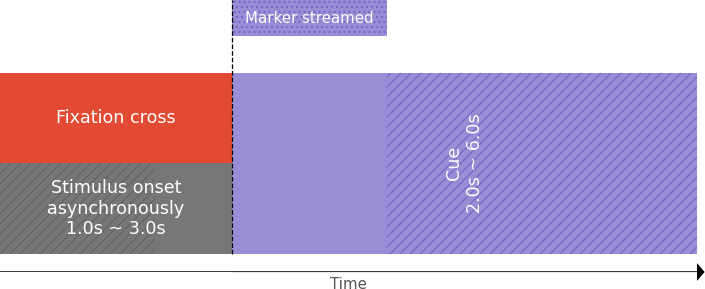
\includegraphics[width=1\textwidth]{Appendix/databases/Figures/mi-paradigm.png}
\par\end{centering}
\caption{\gls*{MI} paradigm implementation with markers indicators.}
\label{}
\end{figure}

%======================================================================
\section{Stimuli presentation}
There is two kind of cues for the \gls{MI} stimuli delivery, the first one is based on the classic arrows and the second one use Pacman-based cues. Both of the paradigms were build with a dashboard that can be used to configure the experiment times.
\begin{figure}[H]
\begin{centering}
% \includesvg[width=0.8\textwidth]{Cap4/Figures/transformer.svg}
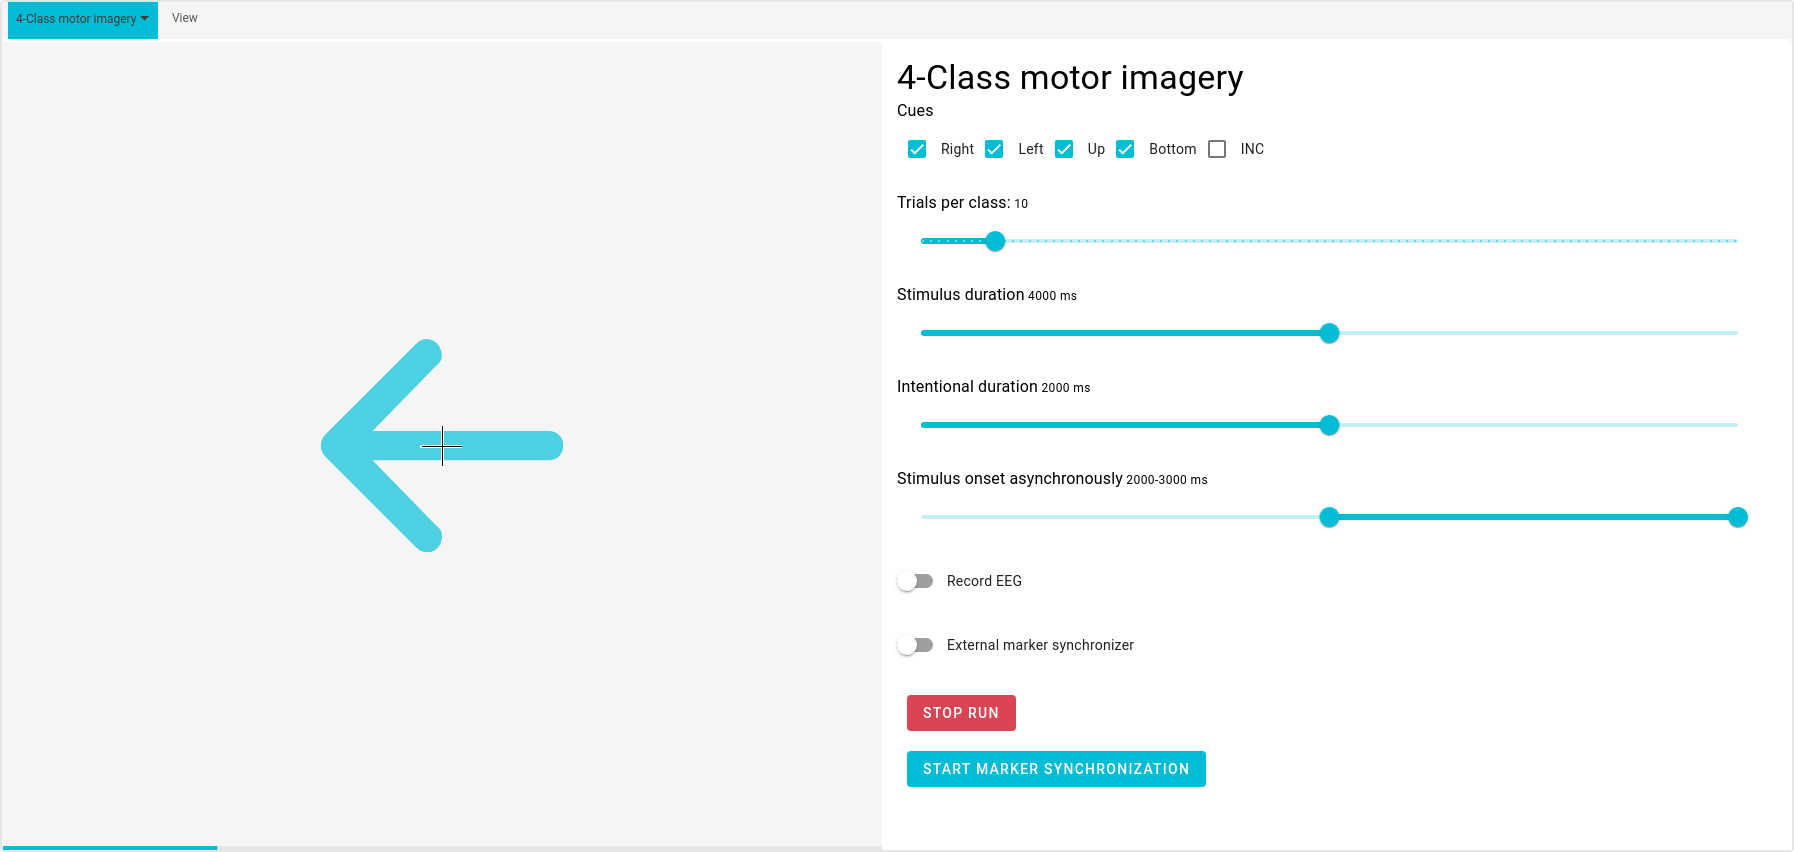
\includegraphics[width=1\textwidth]{Appendix/databases/Figures/mi-delivery.png}
\par\end{centering}
\caption{\gls*{MI} stimuli delivery interface with arrow cues.}
\label{}
\end{figure}

The Pacman-based cues use a clean interface in order to prevent unintentional stimulation, then all screen indicators like time, score, level and bonus were removed. 
\begin{figure}[H]
\begin{centering}
% \includesvg[width=0.8\textwidth]{Cap4/Figures/transformer.svg}
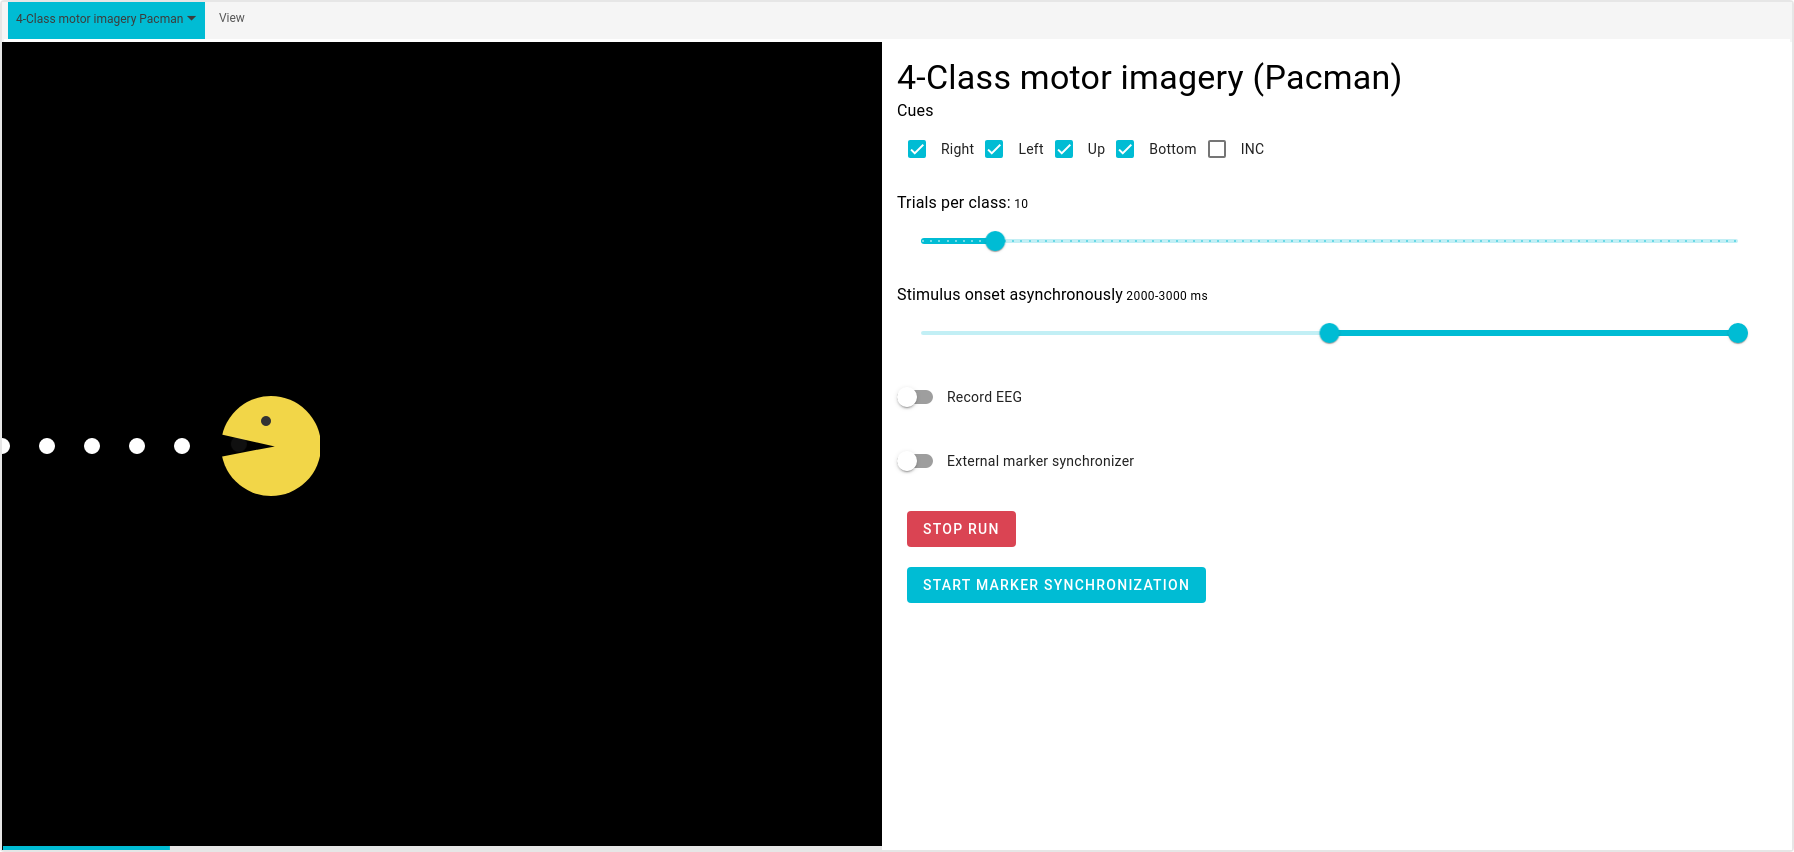
\includegraphics[width=1\textwidth]{Appendix/databases/Figures/mi-delivery-pacman.png}
\par\end{centering}
\caption{\gls*{MI} stimuli delivery interface with pacman-base cues.}
\label{}
\end{figure}


%======================================================================
\section{Intention detection}
An additional feature were included into this paradigm, an intentional detection, the cue add an stimuli indicating the next task, the subject must be instructed about not perform any activity. The intentional detection, this task also has interest in the field of the motor execution.

\begin{figure}[H]
\begin{centering}
% \includesvg[width=0.8\textwidth]{Cap4/Figures/transformer.svg}
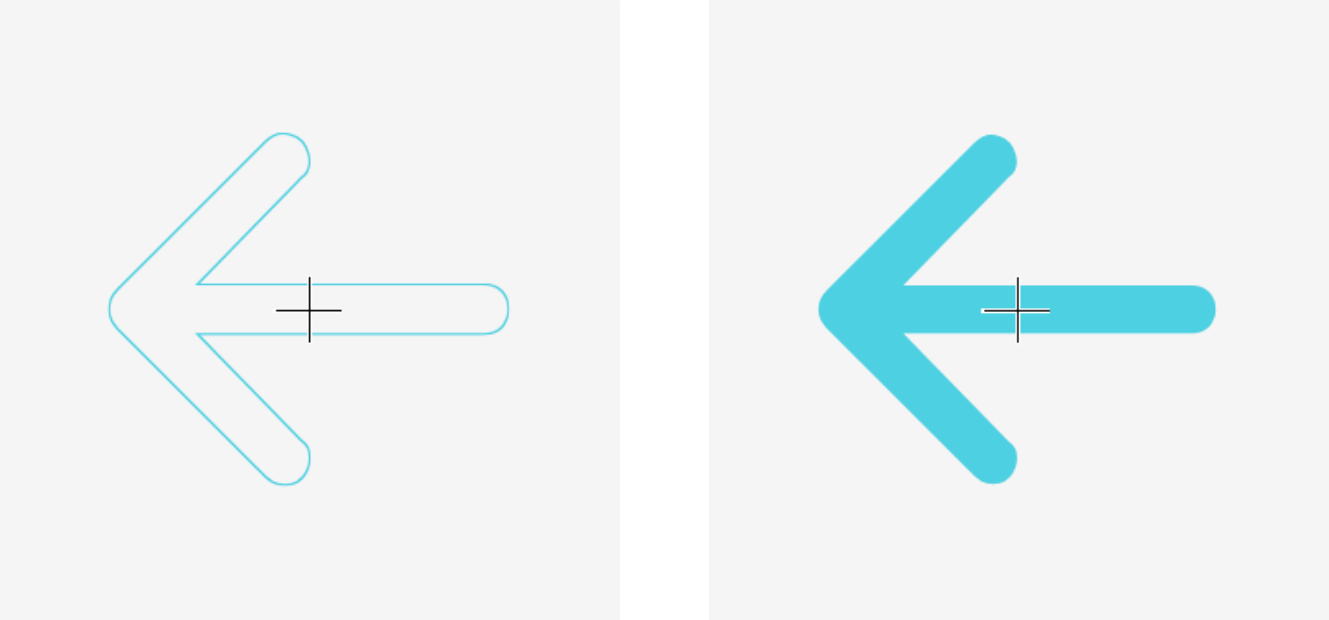
\includegraphics[width=1\textwidth]{Appendix/databases/Figures/mi-intentional.png}
\par\end{centering}
\caption{\gls*{MI} with intentional detection.}
\label{}
\end{figure}

%======================================================================
\section{Motor imagery with intentional non-control stimulus}
Other experimental feature included in the stimuli delivery was the intentional non-control \cite{perdikis2014subject}, this feature is useful to close the loop, since in real implementations there are situations were the patient do not want to perform any action. This new cue is modeled as a circle. 

\begin{figure}[H]
\begin{centering}
% \includesvg[width=0.8\textwidth]{Cap4/Figures/transformer.svg}

\includegraphics[width=1\textwidth]{Appendix/databases/Figures/mi-nonintentional.png}
\par\end{centering}
\caption{\gls*{MI} with nonintentional stimulus.}
\label{}
\end{figure}
